\documentclass[11pt,a4paper]{article}
\usepackage[margin=1in]{geometry}
\usepackage[T1]{fontenc}
\usepackage[utf8]{inputenc}
\usepackage{lmodern}
\usepackage{booktabs}
\usepackage{longtable}
\usepackage{graphicx}
\usepackage{float}
\usepackage{hyperref}
\usepackage{setspace}
\usepackage{enumitem}

\title{Semester Project: Domain Discovery, Recommendation, and Graph Intelligence\\
\large Milestone: Feature Engineering and Dimensionality Reduction (Week 5)}
\author{Iam Anthony Marcelo Alvarez Orellana \\ Jeffrey Ulises Diaz Villanueva \\ Paula Jimena Mancilla Cienfuegos \\ Fernando Samuel Paredes Espinoza}
\date{}

\begin{document}
\maketitle
\onehalfspacing

\section{Prior Milestone Summary}

This report builds on the dataset ingestion and EDA work from Week 3.

\begin{longtable}{p{0.12\linewidth}p{0.25\linewidth}p{0.55\linewidth}}
\toprule
\textbf{Week} & \textbf{Milestone} & \textbf{Key output used here} \\
\midrule
3 & Dataset Charter \& EDA & \texttt{steam\_v1.parquet}: 480,025 interaction records. Star schema on \texttt{AppID}. Games catalog CSV with metadata (tags, genres, price, playtime, etc.). \\
\midrule
\textbf{5} & \textbf{Feature Engineering (this report)} & \textbf{Three feature matrices from catalog. PCA and SVD compression parameters.} \\
\bottomrule
\end{longtable}

\section{Overview}

This milestone covers the construction of the three feature matrices that serve as input to all downstream models (clustering, recommendation, graph analysis), and the dimensionality reduction analysis used to select compression parameters.

All code is in \texttt{src/feature\_engineering.py}. Artifacts are saved to \texttt{artifacts/}. Figures are produced by \texttt{src/generate\_figures.py}.

\section{Dataset Snapshot}

\begin{itemize}[leftmargin=*]
  \item \textbf{Processed dataset:} \texttt{data/processed/steam\_v1.parquet} --- 480,025 user interaction records joined with game catalog on \texttt{AppID}.
  \item \textbf{Games with tag metadata (used for clustering):} 69,943 titles after filtering games with non-empty \texttt{tags} column.
  \item \textbf{Games in feature matrices:} 87,806 titles (full catalog).
\end{itemize}

\section{Feature Matrices Built}

Three complementary representations are constructed, each encoding a different aspect of a game's identity.

\begin{longtable}{p{0.20\linewidth}p{0.22\linewidth}p{0.15\linewidth}p{0.35\linewidth}}
\toprule
\textbf{Matrix} & \textbf{Shape} & \textbf{Type} & \textbf{Content} \\
\midrule
\texttt{X\_numeric} & (87,806 \texttimes{} 26) & Dense & Numerical catalog fields (price, playtime, scores, platform flags, temporal features). Standardized with \texttt{StandardScaler}. \\
\midrule
\texttt{X\_categorical} & (87,806 \texttimes{} 5,000) & Sparse CSR & Top-5,000 genre/category tokens via \texttt{MultiLabelBinarizer}. Binary occurrence encoding. \\
\midrule
\texttt{X\_text} & (87,806 \texttimes{} 5,000) & Sparse CSR & TF-IDF on \texttt{name + short\_description + tags} (1--2 grams, top 5,000 terms). \\
\bottomrule
\end{longtable}

\subsection*{Numeric columns (26)}
Required age, price, DLC count, Metacritic score, achievements, recommendations, user score, score rank, positive/negative review counts, estimated owners, average and median playtime (forever and 2-week windows), peak CCU, percentage positive (total and recent), number of reviews (total and recent), Windows/Mac/Linux flags, release year, release month, and release age in days.

\section{Dimensionality Reduction Analysis}

High-dimensional sparse and dense matrices are impractical for clustering and similarity search. PCA is applied to the dense numeric block, and Truncated SVD is applied to both sparse blocks.

\subsection*{PCA on X\_numeric}

\begin{itemize}[leftmargin=*]
  \item Components tested: up to 26 (full rank).
  \item \textbf{Result:} $k = 12$ components capture $\geq 90\%$ of variance.
  \item Interpretation: 12 orthogonal directions summarize the main axes of variation across games (price tiers, engagement levels, platform availability, recency).
\end{itemize}

\begin{figure}[H]
  \centering
  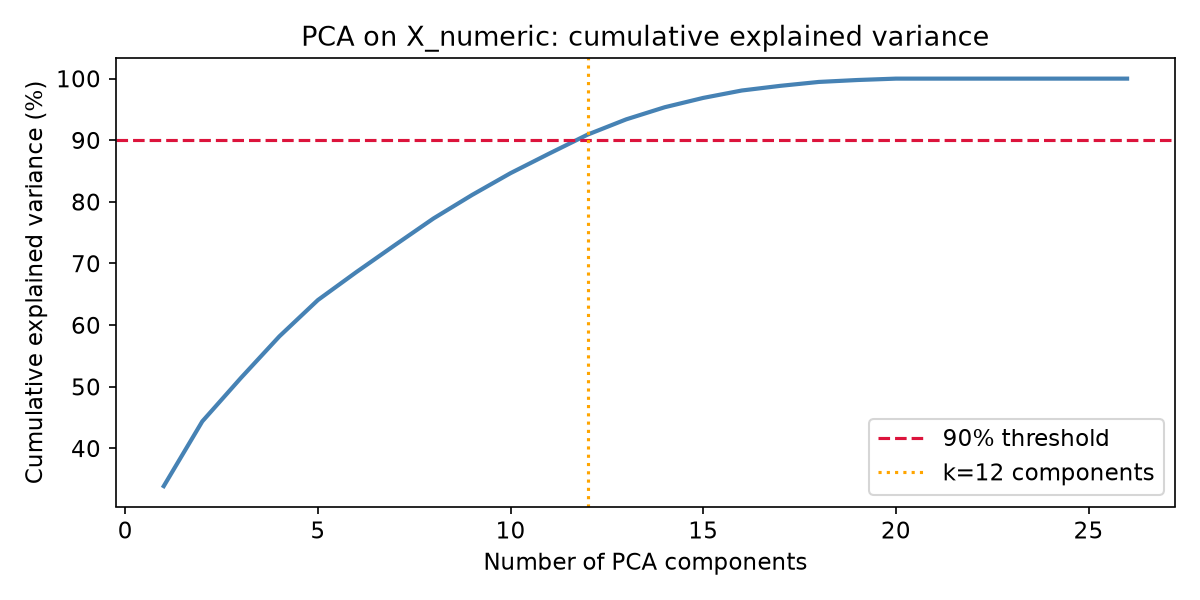
\includegraphics[width=0.85\linewidth]{figs/fig_w5_01_pca_variance.png}
  \caption{PCA on X\_numeric: cumulative explained variance. The dashed red line marks 90\%; the dotted orange line marks $k=12$ components.}
\end{figure}

\subsection*{TruncatedSVD on X\_text}

\begin{itemize}[leftmargin=*]
  \item Components tested: up to 300.
  \item \textbf{Result:} $k = 201$ components capture $\geq 50\%$ of the total squared singular value mass.
  \item Interpretation: text descriptions and tags carry high lexical diversity; 201 latent dimensions are needed before half the signal is concentrated. The singular value spectrum decays slowly (no sharp elbow), typical of document collections with broad vocabulary.
\end{itemize}

\begin{figure}[H]
  \centering
  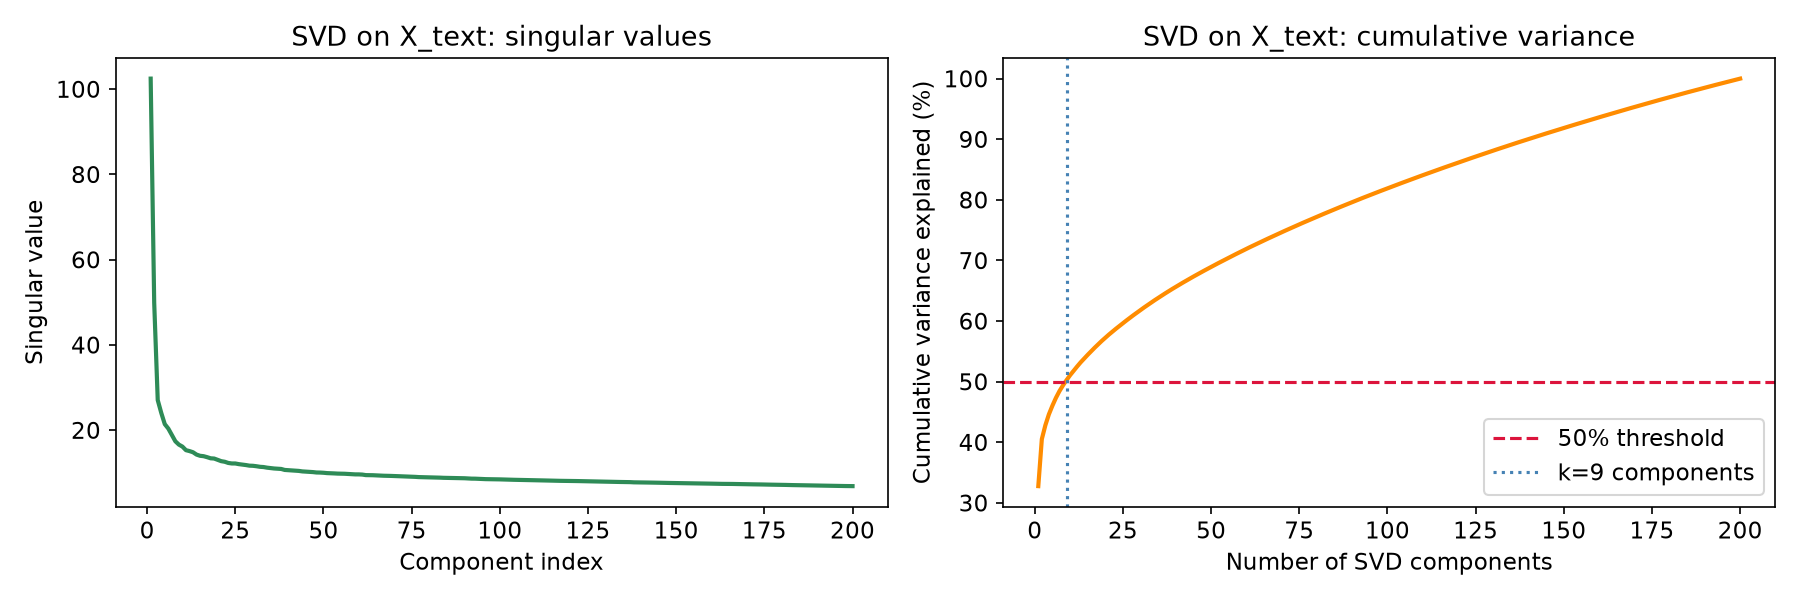
\includegraphics[width=0.95\linewidth]{figs/fig_w5_02_svd_spectrum.png}
  \caption{TruncatedSVD on X\_text: singular value spectrum (left) and cumulative variance explained (right). The dashed red line marks 50\%; dotted line marks $k=201$.}
\end{figure}

\subsection*{Dimensionality Reduction Summary}

\begin{longtable}{p{0.22\linewidth}p{0.18\linewidth}p{0.18\linewidth}p{0.18\linewidth}p{0.16\linewidth}}
\toprule
\textbf{Matrix} & \textbf{Original dims} & \textbf{Reduced dims} & \textbf{Criterion} & \textbf{Method} \\
\midrule
X\_numeric & 26 & 12 & 90\% variance & PCA \\
X\_text & 5,000 & 201 & 50\% variance & TruncatedSVD \\
X\_categorical & 5,000 & 50 (fixed) & downstream use & TruncatedSVD \\
\bottomrule
\end{longtable}

X\_categorical uses a fixed $k=50$ in the clustering pipeline (Week 7), aligned with the tag matrix SVD used there.

\section{Feature Matrix Dimensions}

\begin{figure}[H]
  \centering
  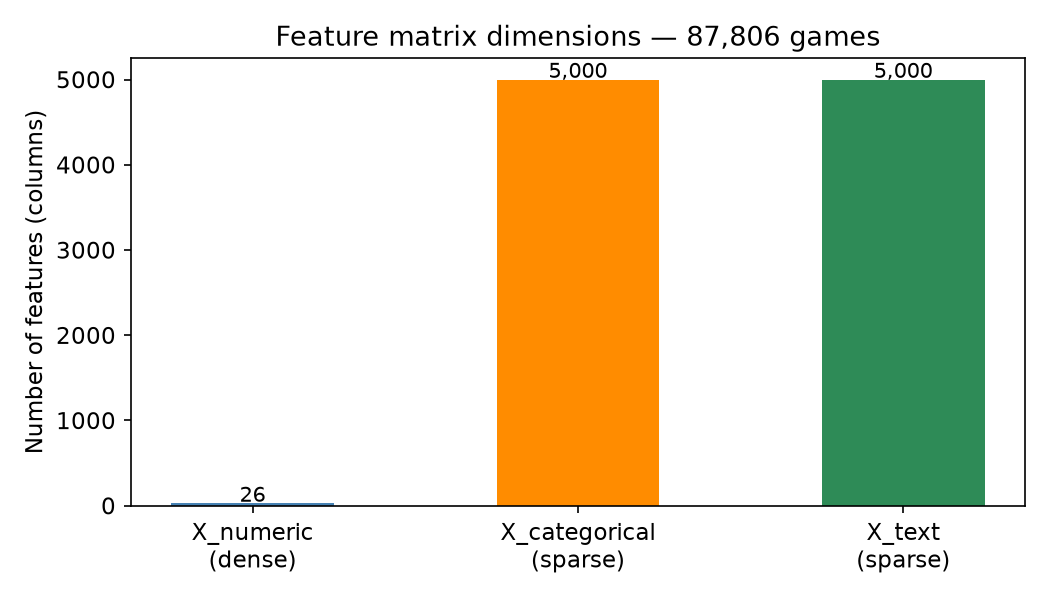
\includegraphics[width=0.75\linewidth]{figs/fig_w5_03_matrix_dims.png}
  \caption{Feature column count per matrix. X\_numeric is the dense analytic block; X\_categorical and X\_text are sparse high-dimensional blocks used for similarity and clustering.}
\end{figure}

\section{Reproducible Pipeline}

\begin{verbatim}
# From project root
python src/feature_engineering.py
\end{verbatim}

Artifacts written to \texttt{artifacts/}:
\begin{itemize}[leftmargin=*]
  \item \texttt{X\_numeric.npz} --- dense numeric matrix (compressed NumPy)
  \item \texttt{X\_categorical.npz} --- sparse categorical matrix (CSR)
  \item \texttt{X\_text.npz} --- sparse TF-IDF text matrix (CSR)
  \item \texttt{models.pkl} --- fitted \texttt{StandardScaler}, \texttt{MultiLabelBinarizer}, \texttt{TfidfVectorizer}, \texttt{PCA}, \texttt{TruncatedSVD} objects
  \item \texttt{metrics.json} --- shapes, PCA/SVD k thresholds, and timestamps
\end{itemize}

All outputs are deterministic (\texttt{random\_state=42}).

\section{Ethics and Access Note}

\begin{itemize}[leftmargin=*]
  \item \textbf{Provenance:} Feature matrices are derived from \texttt{steam\_v1.parquet}, which contains only \texttt{AppID}, game metadata, and interaction counts. No free-text review content, usernames, or personal identifiers are included in the feature matrices.
  \item \textbf{Authorization:} CC0 license; unrestricted academic use.
  \item \textbf{Bias note:} X\_numeric includes \texttt{recommendations} and \texttt{positive} counts, which introduce popularity bias. High-volume AAA games dominate several numeric dimensions. This is noted and will be addressed in the recommendation fairness analysis (Week 10).
\end{itemize}

\end{document}
